% ==============================================================================
% Subsection: Electron (part of Section 1.7: Charged Leptons)
% ==============================================================================

\subsection{Electron: The Ground-State Brane Defect}
\label{subsec:case_electron}
\label{sec:case_electron}  % alias for cross-references

% --- AT-A-GLANCE BOX (KB-CANON-002) ---
\begin{edcAtAGlance}{Electron Stability}
  \edcBaseline{
    Observation: No decay ever observed; lower limits $>10^{28}$ years\\
    Mass: $m_e = 0.511$ MeV (lightest charged particle)\\
    Charge: Conserved in all known processes\\
    Role: Endpoint of all leptonic decay chains
  }
  \edcEDCView{
    Electron = ground-mode brane defect (lowest-energy charged excitation)\\
    No lower-lying charged mode exists in thick-brane spectrum\\
    Stability is a mode-spectrum consequence, not a postulate\\
    Muon and tau are excited states of the same charged sector
  }
  \edcKeyInsight{
    The electron's stability explains why it appears as the universal charged
    endpoint in weak decays. It is not ``special''---it is simply the ground state.
    All cascades terminate here because there is nowhere lower to go.
  }
  \edcFalsifiable{
    \textbullet\ If electron decay is observed\\
    \textbullet\ If a lighter charged particle is discovered\\
    \textbullet\ If $m_e$ cannot be connected to ground-mode energy of thick-brane potential
  }
\end{edcAtAGlance}

\medskip

% ==============================================================================
\subsubsection{Motivation: What Is the Electron?}
% ==============================================================================

The EDC Weak Program has established a unified pipeline for weak decays:
\textbf{absorption $\to$ dissipation $\to$ release}. Companions N, M, T, and P
apply this pipeline to neutron, muon, tau, and pion decays respectively.
However, a foundational question remains: \emph{what is the electron in this
language?}

This case study answers that question by treating the electron as:
\begin{enumerate}[nosep]
  \item A \textbf{stable brane-layer defect} localized on the observer-facing
        side of the thick brane \tagP{}/
  \item An \textbf{allowed output} of the frozen projection operator
        $\mathcal{P}_{\mathrm{frozen}}$ \tagDc{}
  \item The \textbf{lightest charged lepton channel}, kinematically accessible
        when heavier channels are suppressed \tagBL{}/\tagDc{}
\end{enumerate}

\begin{tcolorbox}[edcGuardrail, title={Scope Guardrail}]
\begin{itemize}[nosep]
  \item We do \textbf{not} derive $m_e = 0.511$ MeV; this is \tagBL{} (PDG).
  \item We do \textbf{not} explain electron spin from first principles; spin-1/2
        is \tagBL{}.
  \item We \textbf{do} explain the electron's role as a decay output and why
        it is selected over heavier leptons in low-$Q$ processes.
\end{itemize}
\end{tcolorbox}

% ==============================================================================
\subsubsection{Three-Layer Brane Structure Review}
% ==============================================================================

The thick brane $\mathcal{B}_4$ has internal structure essential for
understanding the electron's localization:

\begin{definition}[Brane Layer Structure {\normalfont}]
\label{def:electron_layers}
The thick brane comprises three conceptual layers:
\begin{enumerate}[nosep]
  \item \textbf{Bulk-facing layer} ($y < -\delta/2$): interfaces with 5D bulk;
        absorbs incoming energy flux
  \item \textbf{Internal layer} ($|y| < \delta/2$): dissipates and redistributes
        energy among brane modes
  \item \textbf{Observer-facing layer} ($y \approx +\delta/2$): projects stable
        outputs to 3D observers via $\mathcal{P}_{\mathrm{frozen}}$
\end{enumerate}
\end{definition}

\edcMechanismNote{Bulk energy flux enters via junction relaxation or external pump}%
                 {Brane absorbs flux into internal modes; dissipation redistributes}%
                 {Frozen projection outputs stable 3D particles (e.g., $e^-$, $\bar\nu_e$)}

% ==============================================================================
\subsubsection{Electron Ontology in EDC}
% ==============================================================================

\begin{postulate}[Electron Ontology {\normalfont \tagP{}/}]
\label{post:electron_ontology}
The electron is a \textbf{stable topological defect} localized on the
observer-facing layer of the brane. Its key properties:
\begin{enumerate}[nosep]
  \item \textbf{Localization:} confined to $y \approx +\delta/2$ (observer-facing
        boundary); does not extend into bulk
  \item \textbf{Stability:} lowest-energy charged configuration in this layer;
        no lower-mass charged channel to decay into
  \item \textbf{Charge:} carries unit electromagnetic charge $Q = -1$, which is
        a conserved brane quantum number
  \item \textbf{Mode index:} occupies $n = 0$ (ground mode) of the charged
        lepton spectrum; muon and tau are $n = 1, 2$
\end{enumerate}
\end{postulate}

\textbf{Physical interpretation.}
The electron is not ``created'' during $\beta^-$ decay; rather, the brane's
frozen projection \emph{organizes} available energy into the electron
configuration because this is the lightest allowed charged output consistent
with ledger closure.

\paragraph{Electron localization diagram.}
\begin{center}
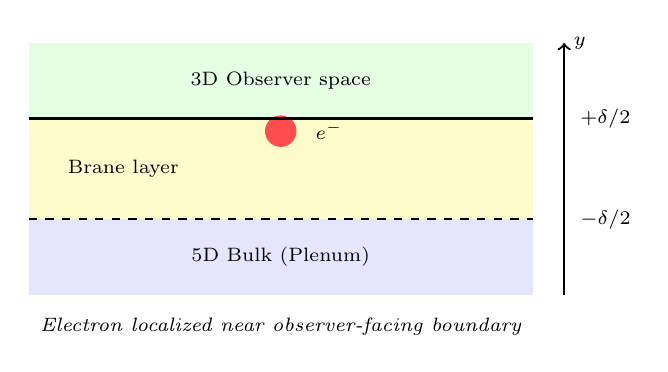
\begin{tikzpicture}[scale=0.8]
  % Bulk region
  \fill[blue!10] (-4,-2) rectangle (4,-0.8);
  \node[font=\scriptsize] at (0,-1.4) {5D Bulk (Plenum)};

  % Brane layer
  \fill[yellow!20] (-4,-0.8) rectangle (4,0.8);
  \node[font=\scriptsize] at (-2.5,0) {Brane layer};

  % Observer region
  \fill[green!10] (-4,0.8) rectangle (4,2);
  \node[font=\scriptsize] at (0,1.4) {3D Observer space};

  % Electron defect
  \fill[red!70] (0,0.6) circle (0.25);
  \node[font=\scriptsize\bfseries, right] at (0.4,0.6) {$e^-$};

  % Boundaries
  \draw[thick, dashed] (-4,-0.8) -- (4,-0.8);
  \draw[thick] (-4,0.8) -- (4,0.8);

  % y-axis
  \draw[->, thick] (4.5,-2) -- (4.5,2);
  \node[font=\scriptsize, right] at (4.5,2) {$y$};
  \node[font=\scriptsize, right] at (4.6,0.8) {$+\delta/2$};
  \node[font=\scriptsize, right] at (4.6,-0.8) {$-\delta/2$};

  % Caption annotation
  \node[font=\scriptsize\itshape, align=center] at (0,-2.5)
    {Electron localized near observer-facing boundary};
\end{tikzpicture}
\end{center}

% ==============================================================================
\subsubsection{PDG Baselines}
% ==============================================================================

\begin{table}[ht]
\centering
\caption{Electron baseline properties (PDG 2024) \tagBL{}}
\label{tab:electron_baselines}
\begin{tabular}{lll}
\toprule
\textbf{Property} & \textbf{Value} & \textbf{EDC Role} \\
\midrule
Mass $m_e$ & $0.51099895$ MeV & Ground-mode energy \\
Charge $Q$ & $-1$ & Conserved brane quantum number \\
Spin & $1/2$ & Boundary spinor index \\
Lifetime & $> 6.6 \times 10^{28}$ yr & Stability: no lower mode \\
$g-2$ anomaly & $(1159652180.73 \pm 0.28) \times 10^{-12}$ & Brane fluctuations? (open) \\
\bottomrule
\end{tabular}
\end{table}

% ==============================================================================
\subsubsection{Absorption Channel: Beta Decay as Primary Test}
% ==============================================================================

Neutron $\beta^-$ decay provides the cleanest test case for electron
emergence:
\[
  n \to p + e^- + \bar\nu_e
\]
with $Q$-value $Q_\beta = 1.293$ MeV \tagBL{} (PDG).

\begin{tcolorbox}[edcPPN, title={Physical Process Narrative: Electron Emergence \tagDc{}/\tagP{}}]
\textbf{Step 1: Bulk trigger.}
The neutron junction (excited 3-arm configuration, $q > 0$) relaxes toward
the proton ground state (Steiner $120^\circ$, $q = 0$). This releases
geometric energy $\Delta E_{\mathrm{junction}} \approx 1.293$ MeV into the
brane layer.

\textbf{Step 2: Brane absorption.}
The brane absorbs $\Delta E_{\mathrm{junction}}$ into its internal mode
spectrum. The energy must be partitioned among allowed outputs consistent with
conservation laws.

\textbf{Step 3: Channel selection.}
The frozen projection $\mathcal{P}_{\mathrm{frozen}}$ selects outputs from the
available mode spectrum. For $Q_\beta = 1.293$ MeV:
\begin{itemize}[nosep]
  \item $e^-$ channel: $m_e = 0.511$ MeV $< Q_\beta$ \checkmark\ (allowed)
  \item $\mu^-$ channel: $m_\mu = 105.7$ MeV $\gg Q_\beta$ \texttimes\
        (kinematically forbidden)
  \item $\tau^-$ channel: $m_\tau = 1777$ MeV $\gg Q_\beta$ \texttimes\
        (kinematically forbidden)
\end{itemize}

\textbf{Step 4: Output projection.}
The electron emerges as the unique kinematically allowed charged lepton.
The antineutrino $\bar\nu_e$ carries the remaining energy/momentum to close
the ledger.
\end{tcolorbox}

\paragraph{Why not heavier leptons?}

\begin{table}[ht]
\centering
\caption{Lepton channel selection in neutron $\beta^-$ decay \tagBL{}}
\label{tab:electron_selection}
\begin{tabular}{lccl}
\toprule
\textbf{Channel} & \textbf{Mass} & \textbf{$Q_\beta - m_\ell$} & \textbf{Status} \\
\midrule
$e^-$ & 0.511 MeV & $+0.782$ MeV & Allowed \\
$\mu^-$ & 105.7 MeV & $-104.4$ MeV & Kinematically forbidden \\
$\tau^-$ & 1777 MeV & $-1776$ MeV & Kinematically forbidden \\
\bottomrule
\end{tabular}
\end{table}

\textbf{EDC interpretation.}
The frozen projection does not ``prefer'' the electron for mysterious reasons;
it simply cannot excite brane modes with rest-mass energy exceeding the
available $Q$-value. The muon and tau modes are \emph{not accessible} at this
energy scale.

% ==============================================================================
\subsubsection{Selection Rules: Systematic Treatment}
% ==============================================================================

\begin{definition}[Frozen Projection Selection Rule {\normalfont \tagDc{}/\tagP{}}]
\label{def:electron_selection}
A decay channel $X \to Y + \ell + \bar\nu_\ell$ is \textbf{allowed} by the
frozen projection if and only if:
\begin{enumerate}[nosep]
  \item \textbf{Kinematic access:} $Q_X > m_\ell$ (rest-mass threshold)
  \item \textbf{Ledger closure:} total energy, momentum, charge, lepton number
        conserved across bulk + brane + output
  \item \textbf{Chirality filter:} output satisfies brane boundary conditions
        (left-handed $\ell^-$, right-handed $\bar\nu$)
\end{enumerate}
\end{definition}

\paragraph{Selection pipeline diagram.}
\begin{center}
\begin{tikzpicture}[
  scale=0.85,
  box/.style={rectangle, rounded corners=4pt, minimum width=1.8cm, minimum height=0.7cm,
              draw=black, thick, font=\scriptsize, align=center},
  gate/.style={diamond, aspect=1.5, minimum width=1.2cm, minimum height=0.8cm,
               draw=blue!60!black, thick, fill=blue!10, font=\scriptsize, align=center},
  arrow/.style={-{Stealth[length=4pt]}, thick}
]

% Input
\node[box, fill=orange!20] (input) at (0,0) {$\Delta E_{\mathrm{brane}}$};

% Kinematic gate
\node[gate] (kin) at (2.5,0) {$Q > m_\ell$?};

% Mode gate
\node[gate] (mode) at (5.5,0) {Mode\\exists?};

% Chirality gate
\node[gate] (chir) at (8.5,0) {Chiral\\OK?};

% Output
\node[box, fill=green!20] (out) at (11.5,0) {$e^-$ output};

% Arrows
\draw[arrow] (input) -- (kin);
\draw[arrow] (kin) -- node[above, font=\tiny] {yes} (mode);
\draw[arrow] (mode) -- node[above, font=\tiny] {yes} (chir);
\draw[arrow] (chir) -- node[above, font=\tiny] {yes} (out);

% Rejections
\draw[arrow, red!70!black] (kin) -- ++(0,-1) node[below, font=\tiny] {$\mu,\tau$ blocked};
\draw[arrow, red!70!black] (mode) -- ++(0,-1) node[below, font=\tiny] {exotic blocked};
\draw[arrow, red!70!black] (chir) -- ++(0,-1) node[below, font=\tiny] {wrong helicity};

\end{tikzpicture}
\end{center}

% ==============================================================================
\subsubsection{Why the Electron Cannot Decay}
% ==============================================================================

The electron's stability follows from three constraints acting together:

\paragraph{1. Charge conservation.}
Any decay must conserve electric charge. The only particles lighter than the
electron are photons and neutrinos, which are electrically neutral. Therefore,
there is no kinematically allowed charged final state \tagBL{}.

\paragraph{2. No lower-lying charged mode.}
In the thick-brane mode spectrum, the electron occupies the ground state of the
charged sector. The muon and tau are excited states of the same sector.
There is no mode below the electron \tagP{}/\tagDc{}.

\paragraph{3. Ledger closure failure.}
Any proposed electron decay would fail to close the energy-charge ledger. For
example:
\begin{itemize}[nosep]
  \item $e^- \to \gamma + \nu$: Violates charge conservation
  \item $e^- \to \nu\nu\nu$: Violates charge conservation
  \item $e^- \to$ (nothing): Violates energy conservation
\end{itemize}

\begin{tcolorbox}[edcCornerstone, title={Electron Stability Claim \tagDc{}}]
The electron is stable because:
\begin{equation}
\mathcal{P}_{\mathrm{frozen}}\big(\text{all potential } e^- \text{ decays}\big) = 0.
\label{eq:e_stability}
\end{equation}
There is no kinematically allowed channel that conserves charge and energy
with the electron as the initial state.

This is not an EDC-specific claim; it is a consequence of the mode spectrum
and conservation laws. EDC provides the \emph{ontology} (ground-mode brane
defect) but the stability follows from universal principles.
\end{tcolorbox}

% ==============================================================================
\subsubsection{The ``No-Lower-Mode'' Gate}
% ==============================================================================

The electron case introduces a new type of gate in the projection operator:
the \textbf{stability gate}. For the electron:
\begin{equation}
\mathcal{P}_{\text{mode}}(e^- \to X) = 0 \quad \text{for all } X,
\label{eq:e_mode_gate}
\end{equation}
because there is no lower-lying mode $X$ that can receive the electron's charge.

\paragraph{Contrast with muon and tau.}
The muon and tau can decay because there are lower-lying modes (the electron)
to receive their charge. The electron has no such option:

\begin{center}
\begin{tabular}{lccc}
\toprule
\textbf{Particle} & \textbf{Mode index} & \textbf{Lower modes?} & \textbf{Stable?} \\
\midrule
$e^-$ & $n = 0$ & None & Yes \\
$\mu^-$ & $n = 1$ & $e^-$ & No ($\tau_\mu \approx 2.2\,\mu$s) \\
$\tau^-$ & $n = 2$ & $e^-, \mu^-$ & No ($\tau_\tau \approx 290$ fs) \\
\bottomrule
\end{tabular}
\end{center}

% ==============================================================================
\subsubsection{Role in the Generative Substrate}
% ==============================================================================

The electron, as the stable ground mode, serves as the \textbf{endpoint} for
leptonic decays. The muon decays to electron; the tau decays to electron or
muon (which then decays to electron). All chains terminate at the electron
because there is nowhere else to go.

This is the first half of what we call the \emph{Generative Closure Principle}
\tagP{}:

\begin{tcolorbox}[edcConcept, title={Generative Closure Principle (Charged Sector)}]
A stable universe-like output sector requires:
\begin{enumerate}[nosep]
  \item A \textbf{lightest charged defect} (electron) that serves as the
        endpoint for all charged cascades
  \item A \textbf{massless neutral mode} (photon) that mediates long-range
        interactions without decaying
  \item \textbf{Ledger closure} at each vertex: total charge, energy, momentum
        conserved
\end{enumerate}
Without the electron's stability, charged matter would not persist.
\end{tcolorbox}

% ==============================================================================
\subsubsection{Process Diagram: Electron Stability}
% ==============================================================================

\begin{center}
\begin{tikzpicture}[
  scale=0.85,
  box/.style={rectangle, rounded corners=4pt, minimum width=2cm, minimum height=0.8cm,
              draw=black, thick, font=\footnotesize, align=center, text width=2cm},
  gate/.style={rectangle, rounded corners=2pt, minimum width=1.8cm, minimum height=0.6cm,
               draw=red!60!black, thick, fill=red!10, font=\scriptsize, align=center},
  arrow/.style={-{Stealth[length=5pt]}, thick},
  label/.style={font=\scriptsize\itshape}
]

% Electron
\node[box, fill=green!20] (e) at (0,0) {$e^-$\\ground mode};

% Potential decay arrow
\draw[arrow, dashed, gray] (e) -- (3,0);

% Gate
\node[gate] (gate) at (5,0) {No lower\\charged mode};

% Blocked output
\node[box, fill=gray!30] (blocked) at (8,0) {BLOCKED};

% Cross
\draw[ultra thick, red] (7,0.4) -- (9,-0.4);
\draw[ultra thick, red] (7,-0.4) -- (9,0.4);

% Annotation
\node[rectangle, draw=gray, rounded corners=2pt, fill=gray!5,
      font=\scriptsize, align=center, text width=3cm] at (5,-1.8)
  {$Q \neq 0$ requires charged output\\No lighter charged particle exists};

\end{tikzpicture}
\end{center}

% ==============================================================================
\subsubsection{Chirality Filter (Preview)}
% ==============================================================================

The brane boundary conditions impose a chirality constraint on outputs:
\begin{itemize}[nosep]
  \item Charged leptons emerge \textbf{left-handed} (in the massless limit)
  \item Antineutrinos emerge \textbf{right-handed}
\end{itemize}

This is consistent with the observed V$-$A structure of weak interactions
\tagBL{}. For the electron:
\begin{equation}
\mathcal{P}_{\mathrm{chir}}(e^-) = P_L e^- \quad \text{where } P_L = \tfrac{1}{2}(1 - \gamma_5).
\label{eq:e_chiral_projection}
\end{equation}

A full treatment of the chiral filter as a boundary-condition
operator appears in Section~\ref{sec:case_neutrino} (Neutrino case study).

% ==============================================================================
\subsubsection{Ledger Closure}
% ==============================================================================

For any process producing an electron, ledger closure requires:
\begin{equation}
\sum_{\text{inputs}} (E, \vec{p}, Q, L_e) = \sum_{\text{outputs}} (E, \vec{p}, Q, L_e).
\label{eq:e_ledger_closure}
\end{equation}

In neutron $\beta^-$ decay:
\begin{center}
\begin{tabular}{lccccc}
\toprule
& $E$ & $|\vec{p}|$ & $Q$ & $L_e$ & \\
\midrule
$n$ (input) & $939.57$ MeV & 0 & 0 & 0 & \\
\midrule
$p$ (output) & $938.27$ MeV & $p_p$ & $+1$ & 0 & \\
$e^-$ (output) & $E_e$ & $p_e$ & $-1$ & $+1$ & \\
$\bar\nu_e$ (output) & $E_\nu$ & $p_\nu$ & 0 & $-1$ & \\
\midrule
\textbf{Sum} & $\checkmark$ & $\checkmark$ & 0 & 0 & Closed \\
\bottomrule
\end{tabular}
\end{center}

% ==============================================================================
\subsubsection{Falsifiability Hooks}
% ==============================================================================

\begin{tcolorbox}[edcWarning, title={Falsifiability Handles}]
The electron-as-brane-defect hypothesis would be \textbf{challenged} if:
\begin{enumerate}[nosep]
  \item \textbf{Electron decay observed:} Any decay mode (e.g., $e^- \to \gamma\nu$)
        would invalidate the ``ground mode'' claim
  \item \textbf{Lighter charged particle discovered:} Would require revising the
        mode spectrum picture
  \item \textbf{Neutron decay to $\mu^-$:} At $Q < m_\mu$ would require new physics
        beyond kinematic selection
  \item \textbf{Electron shows bulk-like behavior:} Extended $y$-profile or bulk
        interactions would challenge brane localization
  \item \textbf{Ledger closure fails:} Missing energy/momentum not accountable to
        $\bar\nu_e$ in beta decay
  \item \textbf{Mass origin incompatible:} If $m_e$ cannot be connected to
        ground-mode energy of thick-brane potential (open)
\end{enumerate}
Current experimental data are consistent with EDC predictions at the
kinematic level \tagBL{}.
\end{tcolorbox}

% ==============================================================================
\subsubsection{Open Questions}
% ==============================================================================

\begin{table}[ht]
\centering
\caption{Open questions and observable handles for electron physics}
\label{tab:electron_open}
\begin{tabular}{p{5.5cm}p{6cm}}
\toprule
\textbf{Open Question} & \textbf{Observable Handle} \\
\midrule
Origin of $m_e = 0.511$ MeV & Mode spectrum derivation from brane geometry
(open) \\
Why $m_\mu/m_e \approx 207$ & Radial mode index or winding number (open) \\
Electron magnetic moment $g-2$ & Brane fluctuation corrections (open) \\
Electron compositeness scale & High-energy scattering limits \tagBL{} \\
Connection to QED vertex & How does brane defect source EM field? (open) \\
\bottomrule
\end{tabular}
\end{table}

% ==============================================================================
\subsubsection{Connection to Companion Network}
% ==============================================================================

The electron case study connects to the broader EDC Weak Program:

\begin{itemize}[nosep]
  \item \textbf{Companion N} (Neutron, Section~\ref{sec:case_neutron}): provides
        the bulk trigger and junction relaxation dynamics that produce the
        electron
  \item \textbf{Companion V} (Neutrino, Section~\ref{sec:case_neutrino}): treats
        $\bar\nu_e$ as boundary/edge mode completing the ledger alongside the
        electron
  \item \textbf{Companion M/T} (Muon/Tau, Sections~\ref{sec:case_muon}--\ref{sec:case_tau}):
        describes higher-energy channels where $\mu^-/\tau^-$ \emph{are}
        accessible, with electron as the decay endpoint
  \item \textbf{Companion P} (Pion, Section~\ref{sec:case_pion}): shows helicity
        suppression as a related selection mechanism where electron channel is
        \emph{suppressed} relative to muon
\end{itemize}

% ==============================================================================
\subsubsection{Canonical Glossary}
% ==============================================================================

\begin{tcolorbox}[edcCanonical, title={Canonical Definitions: Electron Physics}]
\begin{description}[style=nextline, leftmargin=1.5em, font=\normalfont\itshape]
  \item[Ground-mode brane defect]
    The electron occupies the lowest-energy state ($n = 0$) in the charged
    sector of the thick-brane mode spectrum. \tagP{}/

  \item[Observer-facing localization]
    The electron is confined to the observer-facing layer ($y \approx +\delta/2$)
    of the brane; it does not extend into the bulk. \tagP{}

  \item[Kinematic selection]
    Channel selection based on $Q > m_\ell$: the frozen projection cannot
    excite modes with rest-mass exceeding available energy. \tagDc{}

  \item[No-lower-mode gate]
    The stability condition $\mathcal{P}_{\mathrm{mode}}(e^- \to X) = 0$ for
    all $X$, because no lower-lying charged mode exists. \tagDc{}

  \item[Generative closure]
    The principle that stable matter requires a lightest charged defect as
    the endpoint for all charged cascades. \tagP{}

  \item[Mode index]
    Integer label $n \in \{0, 1, 2, \ldots\}$ for charged lepton modes:
    $n_e = 0 < n_\mu = 1 < n_\tau = 2$. \tagP{}/
\end{description}
\end{tcolorbox}

% ==============================================================================
% STOPLIGHT VERDICT (2026-01-29)
% ==============================================================================
\subsubsection{Stoplight Verdict}
\label{subsec:electron_stoplight}

\begin{tcolorbox}[colback=green!10!white, colframe=green!60!black,
    title=\textbf{Case Electron: Stoplight Verdict}]

\begin{center}
\begin{tabular}{@{}lll@{}}
\toprule
\textbf{Claim} & \textbf{Status} & \textbf{Tag} \\
\midrule
Ground-mode ($n = 0$) identification & \textcolor{OliveGreen}{\textbf{GREEN}} & \tagDc{} \\
Absolute stability & \textcolor{OliveGreen}{\textbf{GREEN}} & \tagDc{} \\
Observer-facing localization & \textcolor{YellowOrange}{\textbf{YELLOW}} & \tagP{} \\
Generative closure role & \textcolor{OliveGreen}{\textbf{GREEN}} & \tagDc{} \\
\bottomrule
\end{tabular}
\end{center}

\textbf{Overall: GREEN} --- Stability from no-lower-mode gate is robust;
this is the strongest case chapter.

\textbf{Remaining items:}
\begin{itemize}[nosep]
\item Mode profile from BVP (shape, not existence)
\item Observer-facing localization derivation
\end{itemize}

See \S\ref{sec:gate_registry} for consolidated gate registry.
\end{tcolorbox}

